%%%%%%%%%%%%%%%%%%%%%%%%%%%%%%%% 
\section{The WA105 Prototype} 
\label{sec:proto-cern-double}

In the recent years, two consecutive FP7 Design Studies
(LAGUNA/LAGUNA-LBNO) have led to the development of a conceptual
design (fully engineered and costed) for a 20~kt/50~kt GLACIER-type
underground neutrino detector. In these studies, an underground
implementation has been assumed {\it ab initio} and such constraints
have been important and taken into account in design choices. The
LAGUNA-LBNO design study, completed in August 2014, has produced many
technological developments focused on the construction of large and
affordable liquid argon underground detectors addressing the complete
investigation of 3-flavor neutrino oscillations and the determination
of their still unknown parameters. These detectors will be very
powerful for important non-beam studies such as proton decay,
atmospheric neutrinos and supernovae neutrinos. The WA105 experiment,
approved in 2013, is designed to provide a full scale demonstration of
these technological developments and to characterize the detector
response to hadronic and electromagnetic showers with the detector
exposed to a charged hadron/electron/muon beam with momentum
0.5--20~GeV/c. A detailed description of the experiment is available
in the 2014 Technical Design Report~\cite{WA105_TDR} and an up-to-date
picture of the technical developments in WA105 can be found in the
March 2015 Status Report Document~\cite{WA105_SREP} submitted to the
SPSC CERN committee. These developments are the basis of the DUNE
Alternative Far Detector design and are described in
Chapter~\ref{ch:detectors-fd-alt}.

The WA105 demonstrator is a dual-phase LArTPC with an active
volume of $6\times 6\times 6$~$m^3$. These dimensions are motivated by
the fact that the basic readout component of the large-scale
LAGUNA/LBNO 20--50~kt detectors are $4\times 4$~m$^2$ Charge Readout
Plane (CRP) units.  The $6\times6$~m$^2$ is consistent with having a
fiducial volume corresponding to that readout unit and with a full
containment of hadronic showers.  Surface operation prohibits drift
lengths above 6~m. The footprint of the active volume corresponds to
1:20 of the surface of the LBNO 20~kt detector. The active volume
contains $\sim$300~t of liquid argon. The basic parameters of the
detector are presented in Table~\ref{tab:demo_para} 
\begin{cdrtable}[Main parameters of the WA105 demonstrator]{lcc}{demo_para}{Main parameters of the WA105 demonstrator} 
Liquid argon density & T/m$^3$& 1.38 \\ \toprowrule
Liquid argon volume height & m& 7.6 \\ \colhline
Active liquid argon height& m  & 5.99 \\ \colhline
Hydrostatic pressure at the bottom& bar & 1.03 \\ \colhline
Inner vessel size (WxLxH) &m$^3$ & 8.3 $\times$ 8.3 $\times$ 8.1\\ \colhline
Inner vessel base surface& m$^2$& 67.6 \\ \colhline
Total liquid argon volume& m$^3$ & 509.6 \\ \colhline
Total liquid argon mass & t & 705 \\ \colhline
Active LAr area & m$^2$& 36 \\ \colhline
Charge readout module (0.5 x0.5 m$^2$) & & 36\\ \colhline
N of signal feedthrough & & 12 \\ \colhline
N of readout channels & & 7680\\ \colhline
N of PMT & & 36 \\ 
\end{cdrtable}
and a 3D drawing and two cut views are available in
Figure~\ref{fig:6by6_open}, Figure~\ref{fig:6by6_plan} and
Figure~\ref{fig:6by6_vert}.
\begin{cdrfigure}[Illustration of the  $6\times 6\times 6$~$m^3$  with 
the inner detector inside the cryostat]{6by6_open}{Illustration of the  
$6\times 6\times 6$~$m^3$  with the inner detector inside the cryostat}
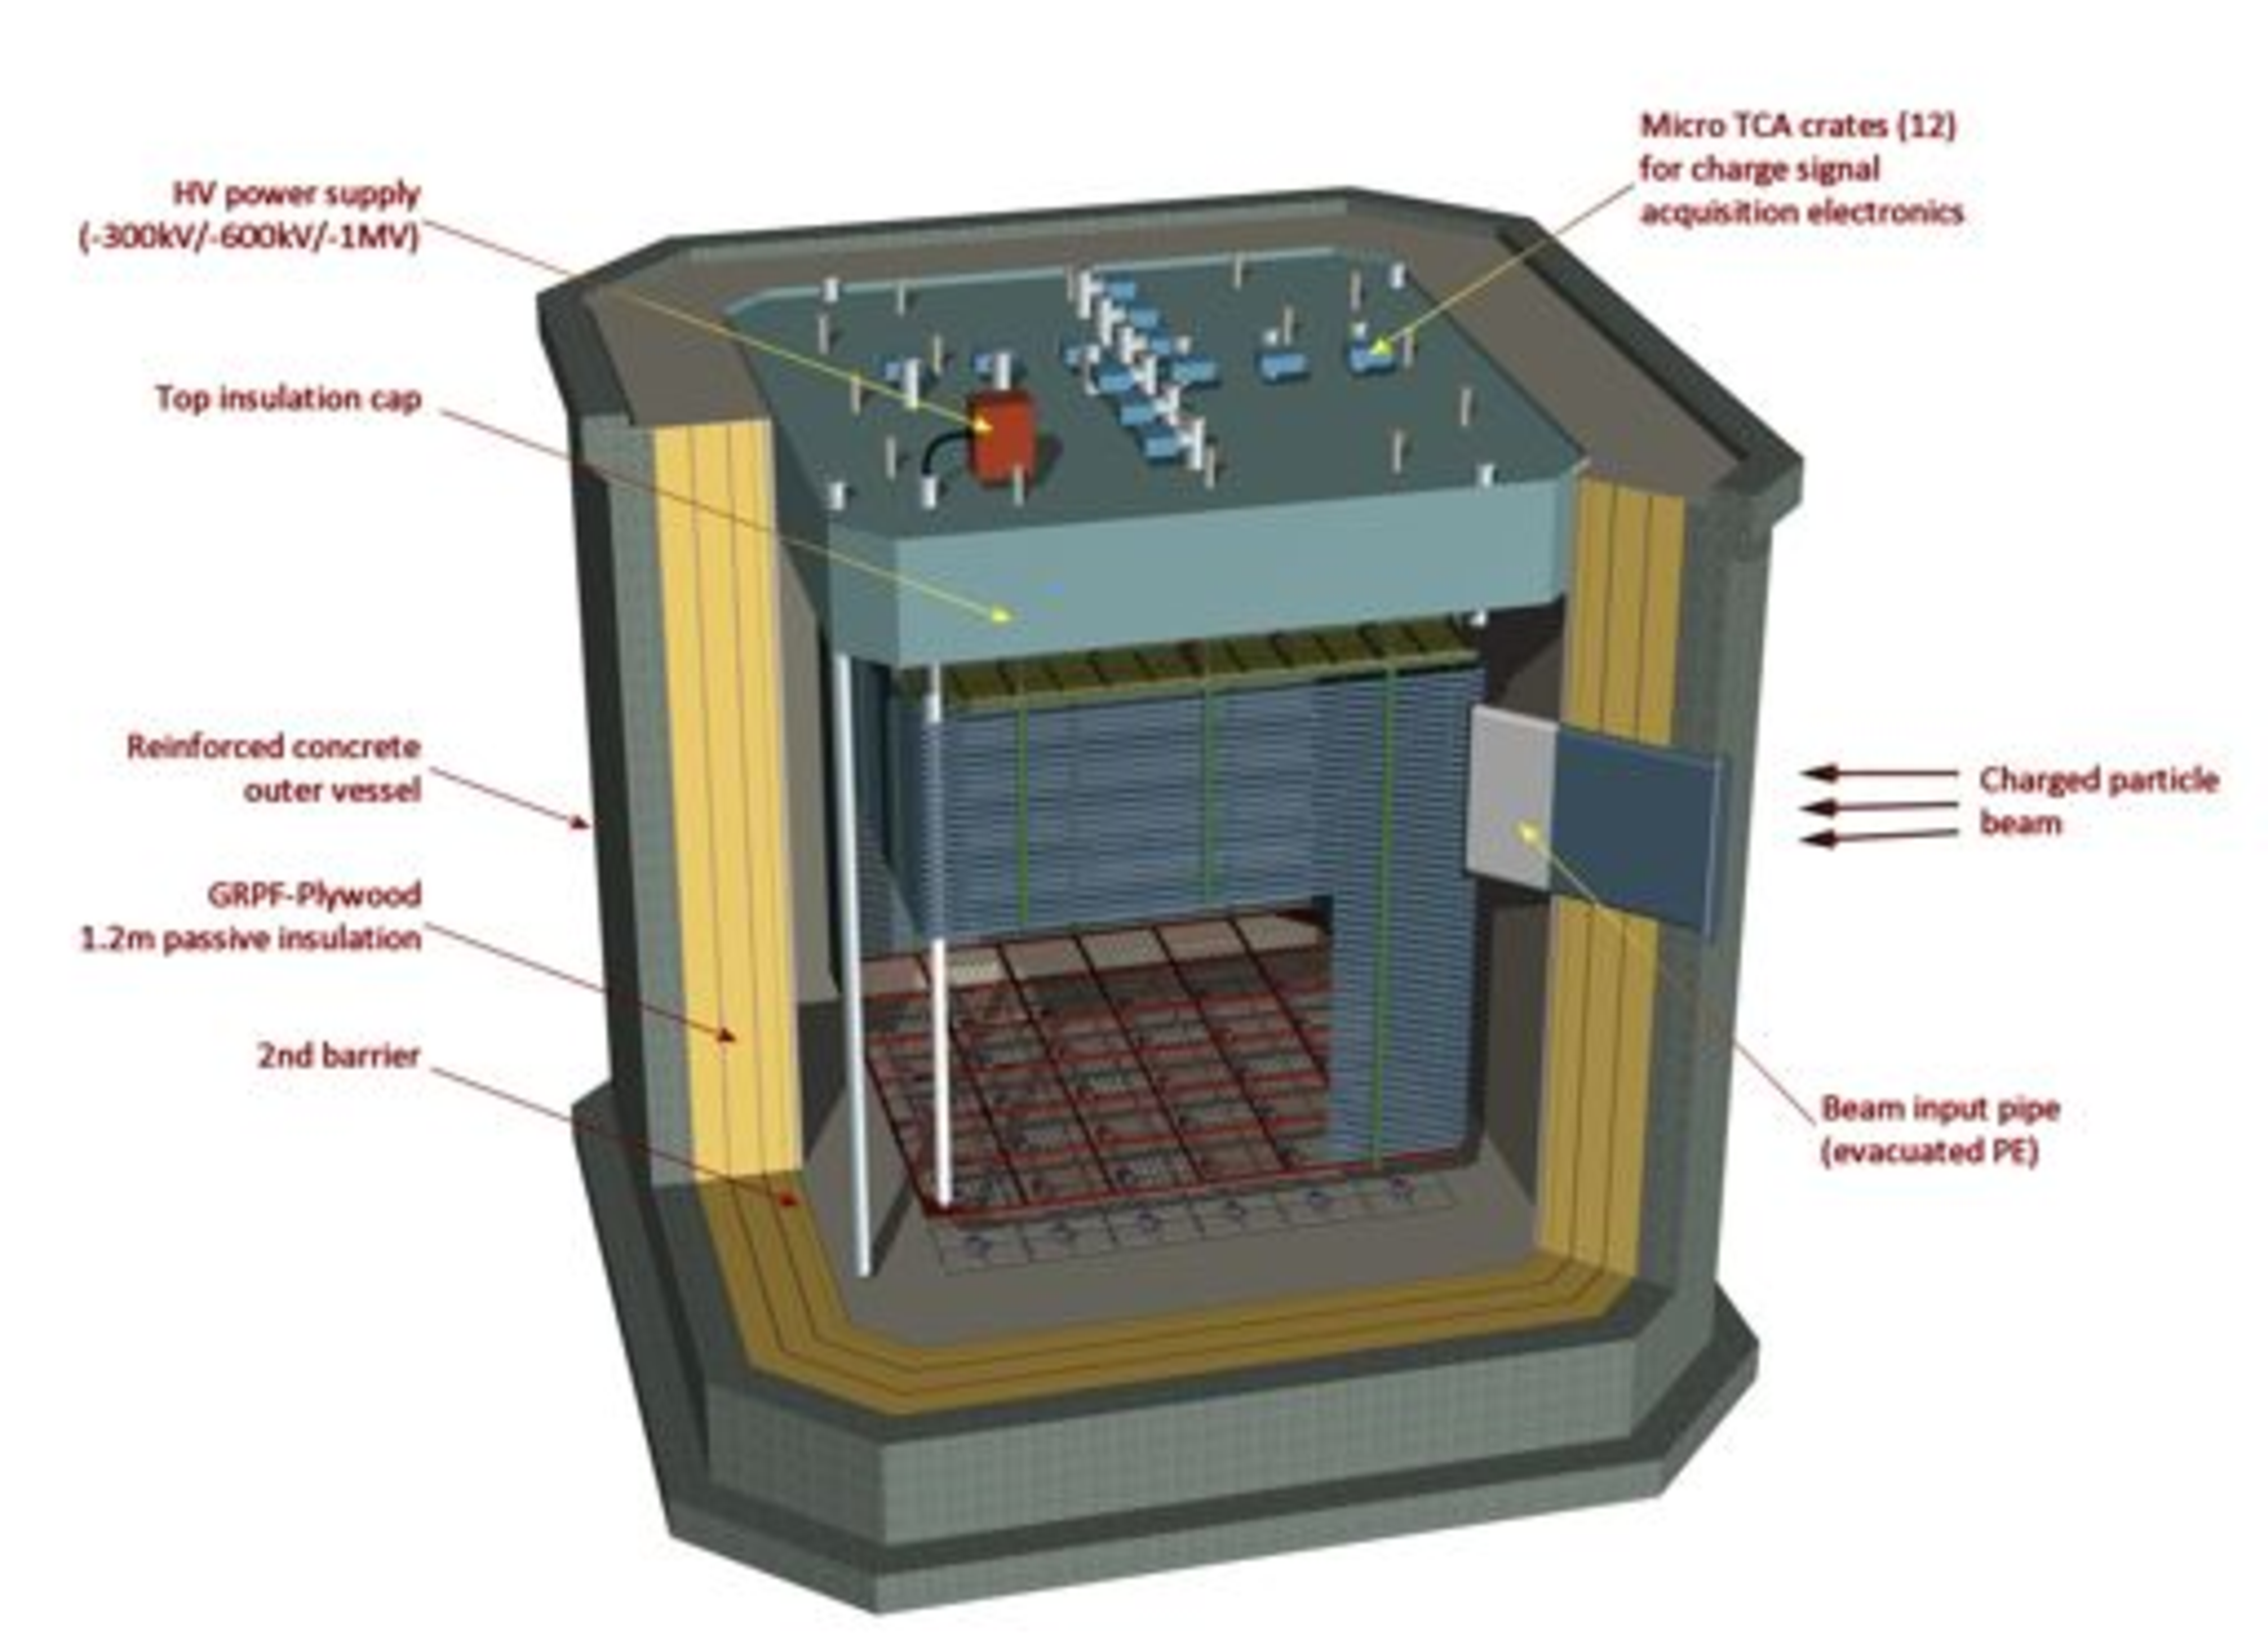
\includegraphics[width=0.7\linewidth]{130618_6x6x6m303v2}
\end{cdrfigure}
\begin{cdrfigure}[Plan view section of the $6\times 6\times 6$~$m^3$]
{6by6_plan}{\small Plan view section of the $6\times 6\times 6$~$m^3$ }
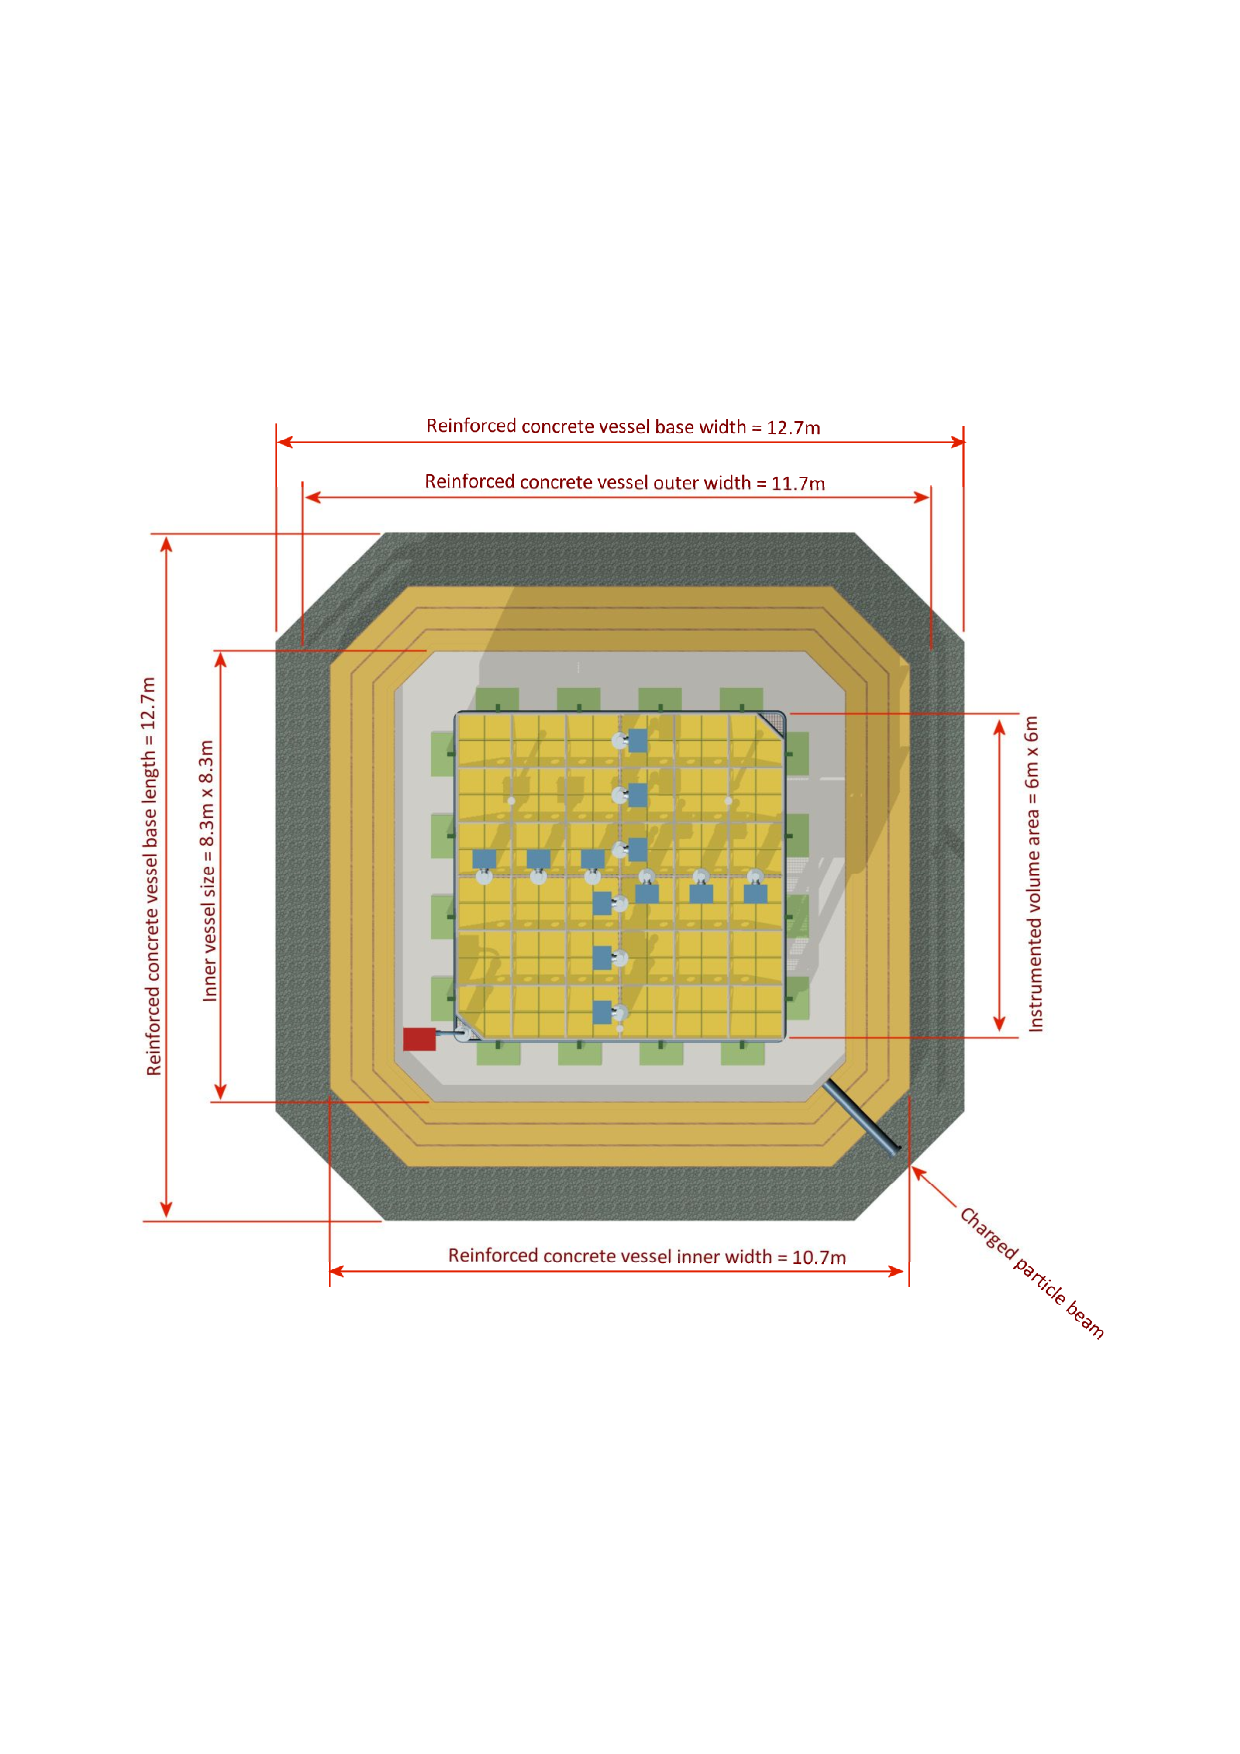
\includegraphics[width=0.7\linewidth]{Detector_overview_horizcross}
\end{cdrfigure}
\begin{cdrfigure}[\small Vertical cross section of the $6\times 6\times 6$~$m^3$]
{6by6_vert}{\small Vertical cross section of the $6\times 6\times 6$~$m^3$}
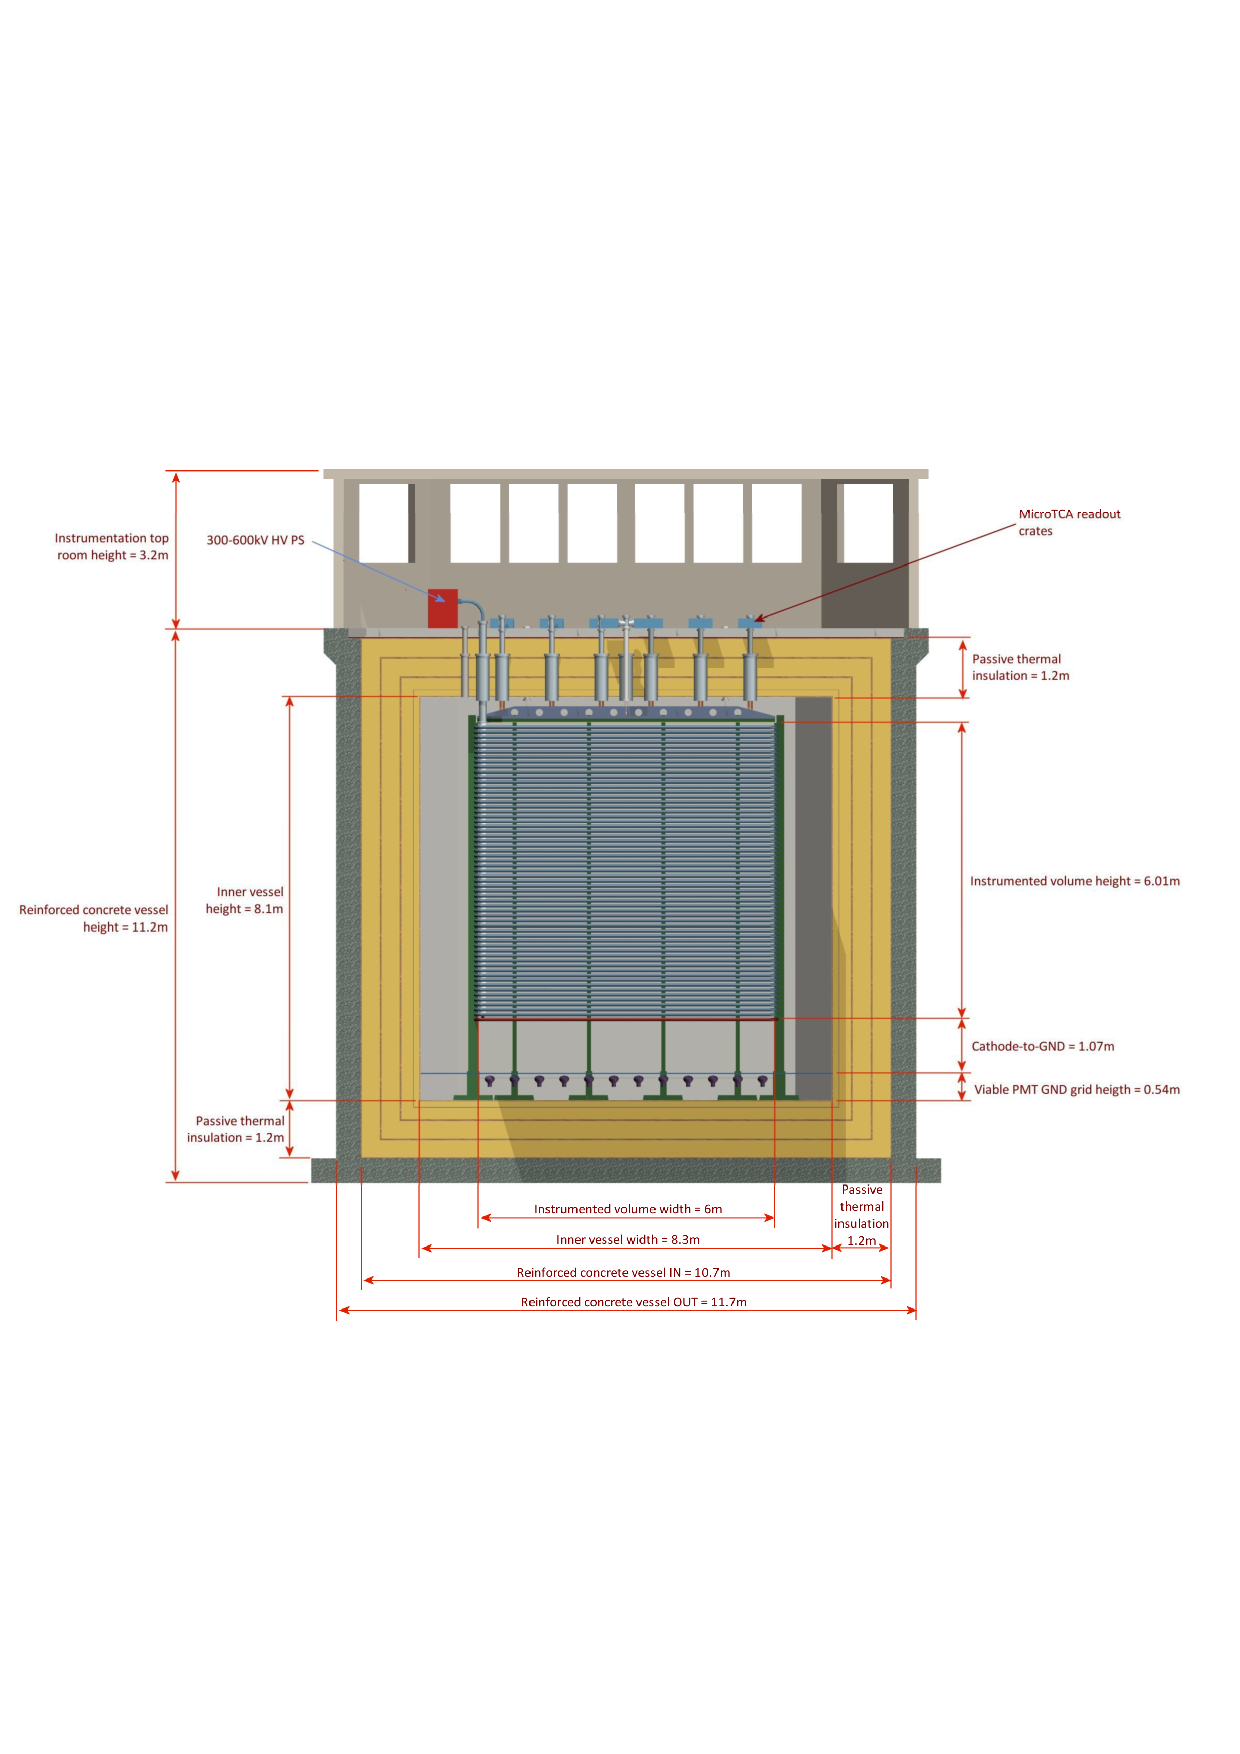
\includegraphics[width=0.7\linewidth]{Detector_overview_verticalcross}
\end{cdrfigure}

The dual-phase LArTPC is based on the vertical drift of the
ionization electrons in LAr in a uniform electric field up to the
liquid-vapor interface, where they are extracted from the liquid into
the gas phase with a higher field made with a submersed grid. The
electrons are then amplified in the GAr due to avalanches occurring
in micro-pattern detector called LEM (Large Electron Multiplier) and
collected on a 2D anode made with a printed circuit board. The
sandwich structure composed by the LEM, Anode and extraction
grid is the CRP. The gain provided by the
amplification in gas allows for the compensation of the charge
attenuation along long drift paths and to achieve a S/N greater than
100 for minimum ionizing particles over the 12~m drift path.The drift path
in the WA105 demonstrator reaches 6~m, the detector is foreseen to
work with a drift field of 0.5~kV/cm and 1~kV/cm, corresponding to a
voltage applied to the cathode respectively of $-$300~kV and $-$600~kV. The
CRP has an active surface of 36~$m^2$ subdivided in strips of 3.125~mm
pitch and 3~m length for a total of 7680 readout channels.

The WA105 detector is supposed to demonstrate all the techniques developed for the 20 and 50~kt LBNO detectors:
\begin{itemize}
\item{Tank construction technique based on the LNG industry with non evacuated vessel}
\item{Purification system}
\item{Long drift}
\item{HV system 300--600 kV, large hanging field cage}
\item{Large area dual-phase charge readout}
\item{Accessible cryogenic front end electronics and cheap data acquisition electronics}
\item{Long term stability of UV light readout}
\end{itemize}

At the same time the $6\times 6\times 6$~$m^3$ exposed to the test-beam line has a rich physics program:
\begin{itemize}
\item{Assess detector performance in reconstructing hadronic
  showers; most demanding task in neutrino interactions}
\item{ Measure hadronic and electromagnetic calorimetry and PID performance}
\item{Full-scale software development, simulation and reconstruction}
\item{Collect high statistic hadronic interaction samples with
  unprecedented granularity and resolution for the study of hadronic
  interactions and nuclear effects}
\item{Assess impact on the physics capabilities of a better
  detector performance wrt single phase LArTPC: high S/N ratio, 3~mm
  pitch, absence of materials in long drift space, two collection
  views, no ambiguities}
\item{Study systematics for the long baseline experiment
  related to the reconstruction of the hadronic system (resolution and
  energy scale), electron identification efficiencies, $\pi^0$
  rejection and particle dE/dx identification for proton decay.}
\end{itemize}

The $6\times 6\times 6$~$m^3$ detector is foreseen to start data
taking in 2018 in the extension of the EHN1 Hall, now under
construction. All components are in an advanced state of
design/prototyping or pre-production. Since submission of the TDR,
completion of the WA105 detector design and preparation for
construction have been progressing very quickly during the last
year. Many technical aspects of the design have benefited from the
pre-production and direct practical implementation of the $3 \times 3
\times 1$~$m^3$ setup (see Fig.~\ref{fig:3by1})
\begin{cdrfigure}[Exploded view of the  $3\times 3\times 1$~$m^3$  prototype]
{3by1}{Exploded view of the  $3\times 3\times 1$~$m^3$  prototype}
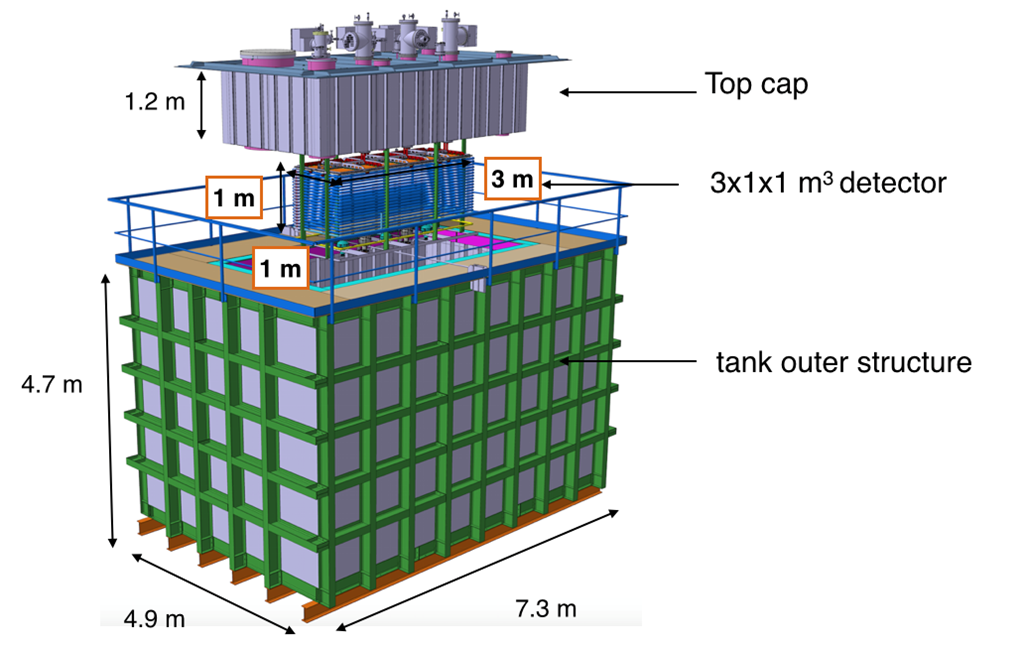
\includegraphics[width=0.95\linewidth]{3by1}
\end{cdrfigure}
which has the minimal size of a readout unit in the final detector.
This allowed a first overview of the complete system integration; a
fully engineered prototype version of many detector parts including
installation details and ancillary services; Quality Assessment (QA),
construction, installation and commissioning plans, to anticipate
legal and practical aspects of the procurement of the different
components and to validate the cost estimations and time schedule for
WA105.  The $3 \times 3 \times 1$~$m^3$ represents a technical
playground and integration exercise to speed up the design,
procurement, QA and commissioning activities needed for the $6\times
6\times 6$~$m^3$ detector.  In particular a complete procedure for the
construction of tanks based on the GTT licensed corrugated membrane
technology has been set up with CERN and a full chain for the
procurement, processing, assembly and commissioning of the LEM
detectors and of the anodes had been also implemented.
